%Si se quiere visualizar la órbita para otro valor del parámetro c, basta con modificar los valores de \cre y \cim.
\documentclass{article}

\usepackage{tikz}
\usepackage{pgfplots}

\begin{document}

\begin{figure}[htbp]
\begin{center}
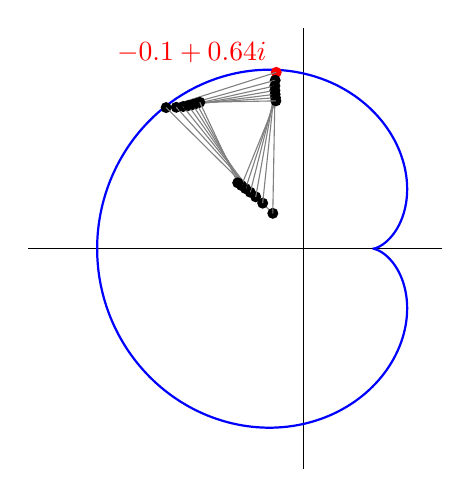
\begin{tikzpicture}[scale=3.5]
% Parámetro c
\def\cre{-0.1}
\def\cim{0.64}

% Ejes
\draw(-1.,0) -- (0.5,0);
\draw  (0,-0.8) -- (0,0.8);

% Cardioide parametrizada
\draw[thick,blue,smooth,domain=0:360,samples=400]
  plot ({0.5*cos(\x) - 0.25*cos(2*\x)},
        {0.5*sin(\x) - 0.25*sin(2*\x)});

\pgfmathsetmacro{\x}{\cre}
\pgfmathsetmacro{\y}{\cim}


% Dibujar punto inicial
 \fill[red](\x,\y) circle (0.02) node[above left] {$\x+\y i$};

% Iteraciones
\foreach \n in {1,...,20} {

    % Calcular z_{n+1}
    \pgfmathsetmacro{\xn}{\x*\x - \y*\y + \cre}
    \pgfmathsetmacro{\yn}{2*\x*\y + \cim}

    % Dibujar segmento
    \draw[gray] (\x,\y) -- (\xn,\yn);

    % Dibujar puntos
    \fill[black] (\xn,\yn) circle (0.02);

    % Actualizar valores
    \xdef\x{\xn}
    \xdef\y{\yn}
}
\end{tikzpicture}
\end{center}
\end{figure}
\end{document}